% Applied Investments 2026 - Portfolio Strategy Project
% HEC Lausanne / UNIL
% Format required by the syllabus: 12pt, 1.5 line spacing, 1-inch margins,
% at most 20 pages excluding tables, graphs and references.
\documentclass[12pt,a4paper]{article}

% Packages
\usepackage[utf8]{inputenc}
\usepackage[T1]{fontenc}
\usepackage[english]{babel}
\usepackage{amsmath,amssymb}
\usepackage{graphicx}
\usepackage{xcolor}
\usepackage{hyperref}
\hypersetup{
    hidelinks
}
\usepackage[margin=1in]{geometry}
\usepackage{setspace}
\usepackage{fancyhdr}
\usepackage{float}
\usepackage{booktabs}
\usepackage{caption}
\usepackage[backend=biber,style=apa,natbib=true]{biblatex}
\DeclareLanguageMapping{english}{english-apa}
\setlength\bibitemsep{0.5\baselineskip}
\addbibresource{references.bib}

\onehalfspacing
\captionsetup{font=small,labelfont=bf,skip=6pt}

% Notes under tables and figures (single-spaced, small)
\newcommand{\tablenote}[1]{\par\vspace{4pt}\begin{minipage}{\linewidth}\footnotesize\singlespacing #1\end{minipage}}

% Header and footer
\setlength{\headheight}{15pt}
\pagestyle{fancy}
\fancyhf{}
\rhead{Applied Investments}
\lhead{Portfolio Strategy Project}
\rfoot{Page \thepage}

% Title page information
\title{%
    \Large \textbf{Applied Investments} \\
    \vspace{0.5cm}
    \LARGE \textbf{Cheap, Cash-Profitable and Correctly Measured: Industry-Relative Value and Quality with Intangible Capital} \\
    \vspace{0.3cm}
    \large \textit{Research question: Does value and quality, measured within industries and corrected for intangible capital, earn an alpha after trading costs?} \\
    \vspace{0.3cm}
    \large Portfolio Strategy Project
}
\author{%
    \normalsize\begin{tabular}{cc}
    Marco D'Amico (25416579) & Roberto Berardi (25419094) \\
    Cedric Nim (XXXXXXXX) & Viola Brignoli (XXXXXXXX) \\
    Ana Luc\'ia Clavijo Mart\'inez (XXXXXXXX) & Claudio Marcoli (XXXXXXXX) \\
    \end{tabular}\\[10pt]
    \small Prof.\ Amit Goyal, HEC Lausanne, University of Lausanne
}
\date{November 2026}

\begin{document}

\maketitle
\thispagestyle{empty}

\newpage
\thispagestyle{empty}
\begin{abstract}
\noindent
This project asks whether a long-short US equity strategy built on value and quality can earn an
alpha against modern factor models after realistic trading costs. We buy stocks that are cheap
relative to their industry and generate high cash-based operating profits, after correcting book
value, assets and profits for the intangible capital that accounting expenses, and we short the
opposite. Cheapness is measured at the current market price and portfolios are formed every three
months. Taken together, the corrections lower the part of the return that the factors explain: from a plain
value-and-quality sort to the final strategy, the net six-factor alpha rises from 0.24\% to 0.53\%
per month and the q5 alpha from 0.06\% to 0.41\%. Over 1963--2015 the value-weighted strategy earns
0.33\% per month after trading costs, and on a 2016--2025 holdout evaluated once it earns 0.73\%,
with a q5 alpha of 0.58\%. The strategy is negatively correlated with the market, pays off in
crises, survives placebo and random-sample tests and remains profitable for a fund of up to about
\$500 million per side.
\end{abstract}

\vspace{0.5cm}
\noindent\textbf{Keywords:} Value; Quality; Intangible capital; Industry-relative characteristics; Factor models; Trading costs

\newpage
\begin{singlespace}
\tableofcontents
\end{singlespace}
\thispagestyle{empty}

\newpage
\pagenumbering{arabic}

% =====================================================================================
\section{Introduction}\label{sec:intro}

\subsection{Economic motivation}

Value and profitability are among the most studied predictors of stock returns. Cheap stocks have
earned more than expensive ones since the early studies of the value premium, and profitable firms
more than unprofitable ones. Both effects, however, are now priced by the factor models that asset
managers use as benchmarks: HML, RMW and CMA in the Fama-French models, and the investment, return
on equity and expected growth factors in the q-factor models. A strategy that simply buys cheap and
profitable stocks therefore earns factor returns, not alpha.

Our starting point is that the usual way of measuring value and quality has three problems.
First, valuation ratios differ across industries for reasons unrelated to mispricing: a bank always
looks cheap next to a software firm, so a market-wide value portfolio is largely an industry bet.
Second, accounting treats investment in research and development, brands and organisation as a cost
rather than as an asset, so book equity, total assets and profits are wrong precisely for the firms
whose value rests on intangible assets. Third, the standard Fama-French convention measures
cheapness with the market price of December of the previous year, so the price is between seven and
eighteen months old when the portfolio is held. If these measurement errors are not captured by the
factors, correcting them should produce returns that the factor models cannot explain.

\subsection{The research question}

We ask whether value and quality, measured within industries, corrected for intangible capital and
at current prices, earn an alpha against the CAPM, the Fama-French five- and six-factor models and
the q5 model, after the costs of trading the strategy. Because the strategy is meant to be run by a
fund, we evaluate it from a fund manager's perspective: value-weighted portfolios of liquid stocks,
explicit trading costs that depend on the size of the fund, and a holdout period that was not used
to design the strategy.

\subsection{Main results and contribution}

Over 1963--2015 the value-weighted long-short spread earns 0.33\% per month net of costs
($t=2.61$), with net alphas of 0.53\% against the six-factor model ($t=3.77$) and 0.41\% against q5
($t=2.58$). On the 2016--2025 holdout, evaluated once after the rules were fixed, the net return is
0.73\% per month and the q5 alpha 0.58\% ($t=2.41$). Building the strategy one correction at a
time shows where this alpha comes from: a plain value-and-quality sort earns the highest raw return,
but almost all of it is factor exposure, and every correction raises the six-factor and q5 alphas.

Our contribution is to combine three corrections that the literature has studied separately
(industry-relative characteristics, intangible capital and timely prices) in one implementable
strategy, to show how much each adds, and to evaluate the result against the hardest benchmark,
the q5 model, net of an explicit cost model and on a holdout period.

\subsection{Report structure}

Section~\ref{sec:lit} reviews the literature, Section~\ref{sec:data} describes the data and
Section~\ref{sec:method} the methodology. Section~\ref{sec:results} presents the results, including
the step-by-step construction and the holdout, and Section~\ref{sec:robust} the robustness tests.
Section~\ref{sec:limits} discusses the limitations and Section~\ref{sec:conclusion} concludes.

% =====================================================================================
\section{Literature review}\label{sec:lit}

\subsection{The value premium and industry-relative characteristics}

The value premium, the higher return of stocks with low prices relative to fundamentals, is one of
the oldest results in empirical finance \citep{FamaFrench1992,LakonishokShleiferVishny1994}.
Valuation ratios, however, differ systematically across industries. \citet{AsnessPorterStevens2000}
show that firm characteristics measured relative to the industry predict returns better than the raw
characteristics, because most of the information in cheapness concerns a firm relative to its
peers. We follow this idea and rank every characteristic within the twelve Fama-French industries.

\subsection{Profitability, cash flows and quality}

Cheap stocks are often cheap for a reason. \citet{NovyMarx2013} shows that profitable firms earn
higher returns than unprofitable ones despite being more expensive, so that combining profitability
with value keeps the cheap firms that are also productive. \citet{AsnessFrazziniPedersen2019}
generalise this idea to a quality factor. On the measurement of profits, \citet{Sloan1996} shows
that investors overweight the accrual part of earnings, and
\citet{BallGerakosLinnainmaaNikolaev2016} find that cash-based operating profitability, which removes
accruals from operating profits, predicts returns better than accounting profitability. Our quality
measure is cash-based operating profitability.

\subsection{Intangible capital}

Expenditures on research and development, brands, customer relationships and organisation create
long-lived assets, but accounting expenses them immediately, so book equity and assets understate
the capital of intangible-intensive firms and current profits understate their profitability
\citep{LevSougiannis1996,ChanLakonishokSougiannis2001}. \citet{PetersTaylor2017} rebuild knowledge
and organisation capital with the perpetual inventory method, and
\citet{EisfeldtKimPapanikolaou2022} show that a value factor based on book equity plus intangible
capital performs better than the standard HML factor, in particular in recent decades. Without this
correction, a value-and-quality strategy systematically shorts healthy pharmaceutical and technology
firms.

\subsection{Timely prices}

The Fama-French convention measures book-to-market with the market value of December of the
previous year. \citet{AsnessFrazzini2013} show that using the current price gives a more timely
value measure that performs better, in particular in combination with momentum. We apply the same
idea to our intangible-adjusted ratios.

\subsection{Factor models, trading costs and out-of-sample evidence}

Because the strategy combines characteristics related to known factors, we measure its performance
against models that contain them: the three-, five- and six-factor models of
\citet{FamaFrench1993,FamaFrench2015,FamaFrench2018}, the last adding momentum
\citep{JegadeeshTitman1993,Carhart1997}, and the q-factor models of \citet{HouXueZhang2015} and
\citet{HouMoXueZhang2021}, whose expected-growth factor makes q5 the hardest benchmark for
profitability-based strategies. Trading costs eliminate the profits of many anomalies
\citep{NovyMarxVelikov2016}, so all our results are net of an explicit cost model. Finally, many
anomalies weaken after publication \citep{McLeanPontiff2016} and many published ones are likely false
positives \citep{HarveyLiuZhu2016}; this is why we keep a holdout period and test the robustness of
the results.

% =====================================================================================
\section{Data}\label{sec:data}

\subsection{Sources and sample}

We use the CRSP monthly stock file and the CRSP/Compustat merged annual fundamentals from WRDS, from
July 1963 to December 2025. The universe contains US common stocks of US-incorporated corporate
issuers listed on NYSE, AMEX and NASDAQ, excluding funds and REITs. Delisting returns are included in
the CRSP returns. For the main tests we exclude microcaps, defined as stocks below the 20th
percentile of NYSE market capitalisation, because their alphas cannot be captured at a realistic
size; the version with microcaps is a robustness test. Factor returns come from Kenneth French's data
library (market, SMB, HML, RMW, CMA, momentum and short-term reversal) and from the q-factor data
library (q5 factors, available from January 1967).

\subsection{Variables and construction}

Compustat data are linked to CRSP with primary and reliable link types and use standard,
consolidated, domestic industrial data. Book equity follows Fama and French: stockholders' equity
plus deferred taxes minus preferred stock, missing if not positive. Accounting data of the fiscal year
ending in calendar year $t-1$ are used from July of year $t$ to June of year $t+1$, so every number
is at least six months old and was public when the portfolio is formed. Market capitalisation is
measured at the firm level, adding all share classes of the same company. Industries are the twelve
Fama-French industries, assigned from the CRSP SIC code.

Beyond the common dataset, our signal needs research and development (\texttt{xrd}), selling,
general and administrative expenses (\texttt{xsga}), goodwill (\texttt{gdwl}), EBITDA
(\texttt{oibdp}), debt and cash for the enterprise value, and receivables, inventories and payables
with their previous-year values. For trading costs we add the CRSP daily file, from which we take
each stock's closing bid and ask at every month end and its trading volume.

\subsection{Descriptive statistics}

Table~\ref{tab:sample} shows the number of stocks in the sorted universe: from about 740 in the
1960s, when the sample is mostly NYSE stocks, to about 2,000 in the 1990s and 1,700 in the holdout
period. Deciles use NYSE breakpoints, so the extreme deciles contain between about 70 and 240 stocks.

\begin{table}[H]
\centering
\caption{Sample: number of stocks sorted each month}\label{tab:sample}
\begin{tabular}{lrrrrrr}
\toprule
Period & Months & Stocks (mean) & Min & Max & Decile 10 & Decile 1 \\
\midrule
1963--1969 & 78 & 738 & 441 & 946 & 73 & 80 \\
1970--1979 & 120 & 1,266 & 935 & 1,457 & 126 & 136 \\
1980--1989 & 120 & 1,540 & 1,449 & 1,651 & 139 & 179 \\
1990--1999 & 120 & 2,032 & 1,626 & 2,456 & 178 & 242 \\
2000--2009 & 120 & 1,876 & 1,577 & 2,584 & 162 & 230 \\
2010--2015 & 72 & 1,643 & 1,573 & 1,817 & 154 & 179 \\
2016--2025 (holdout) & 120 & 1,718 & 1,611 & 1,937 & 163 & 206 \\
\bottomrule
\end{tabular}

\tablenote{Average, minimum and maximum number of stocks with a signal in the main universe (NYSE,
AMEX and NASDAQ common stocks above the 20th NYSE size percentile), and average number of stocks in
the long (decile 10) and short (decile 1) portfolios.}
\end{table}

Table~\ref{tab:legs} describes what the strategy holds. Compared with the short leg, the long leg
has a higher book-to-market, especially once intangible capital is counted, a much higher return on
assets and a much lower past return, consistent with its negative momentum loading
(Section~\ref{sec:behaviour}). The long leg also holds more intangible capital: once intangibles are
counted, intangible-intensive firms are no longer pushed into the short leg. Both legs have a median
size close to that of the median sorted stock.

\begin{table}[H]
\centering
\caption{Characteristics of the long and short portfolios, 1963--2015}\label{tab:legs}
\resizebox{\textwidth}{!}{\begin{tabular}{lrrr}
\toprule
 & Short (decile 1) & Long (decile 10) & All sorted stocks \\
\midrule
Market capitalisation (\$bn) & 0.57 & 0.61 & 0.70 \\
Book-to-market & 0.48 & 0.74 & 0.57 \\
Book-to-market with intangible capital & 0.58 & 1.00 & 0.74 \\
Return on assets (\%) & 2.40 & 8.14 & 5.35 \\
Intangible capital / total capital (\%) & 6.65 & 14.49 & 12.60 \\
Firms reporting R\&D (\%, mean) & 25.38 & 33.38 & 31.50 \\
Past return, months $-12$ to $-2$ (\%) & 21.06 & 2.81 & 13.12 \\
\bottomrule
\end{tabular}
}
\tablenote{Median characteristic of the stocks in each group at each formation date, averaged over all
formation dates from 1963 to 2015. Book-to-market with intangible capital uses $BE - \text{goodwill} +
K + O$ (Section~\ref{sec:method}). Intangible capital over total capital is $(K+O)/(\text{total
assets}+K+O)$. Firms reporting R\&D is an average share, not a median. Market capitalisation and
book-to-market use the current price.}
\end{table}

Ranking within industries gives every industry the same share of its stocks in each decile, but not
the same share of the value of each leg, because the largest firms of an industry can fall on one
side. Figure~\ref{fig:industries} shows the industry weights of the two value-weighted legs and of the
sorted universe. The legs are therefore not industry-neutral by value: the long leg overweights energy
(21\% against 12\% of the sorted universe) and the short leg finance (26\% against 10\%).

\begin{figure}[H]
\centering
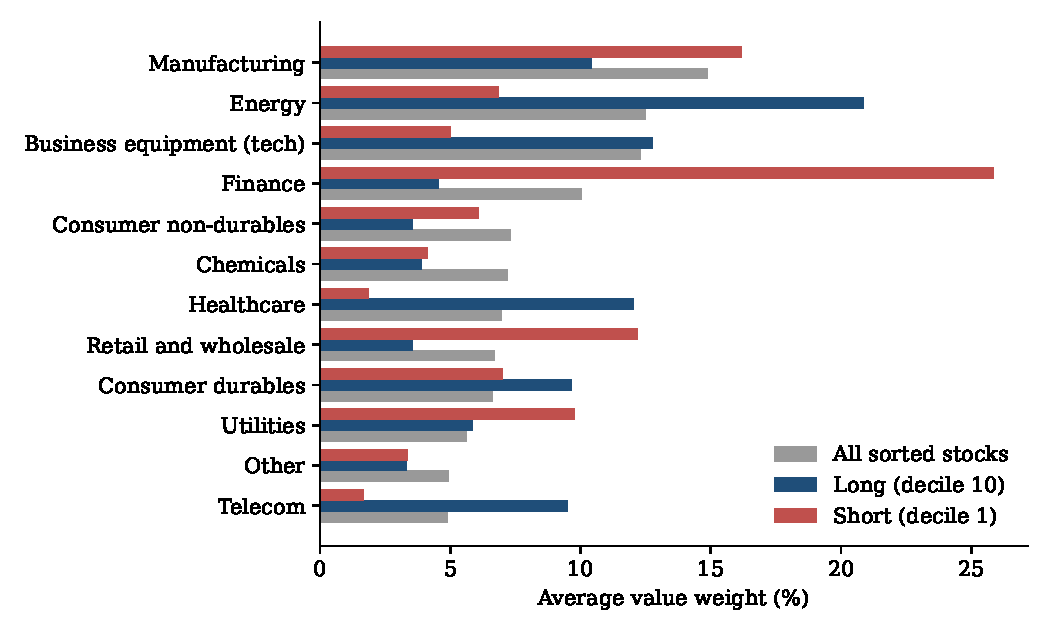
\includegraphics[width=0.9\textwidth]{figures/fig_industries}
\caption{Average value weight of each Fama-French industry in the sorted universe, the long leg
(decile 10) and the short leg (decile 1), 1963--2015 (\%).}\label{fig:industries}
\end{figure}

% =====================================================================================
\section{Methodology}\label{sec:method}

\subsection{Intangible capital}

For every firm and fiscal year we build knowledge capital $K$ and organisation capital $O$ with the
perpetual inventory method of \citet{PetersTaylor2017}:
\begin{align}
K_t &= (1-0.15)\,K_{t-1} + \text{R\&D}_t, \\
O_t &= (1-0.20)\,O_{t-1} + 0.30 \times \text{SG\&A}^{\text{ex R\&D}}_t ,
\end{align}
where SG\&A$^{\text{ex R\&D}}$ is SG\&A minus R\&D (Compustat includes R\&D in SG\&A) and missing
items count as zero. In a firm's first year the capital is set to its steady-state value with 10\%
growth, $K = \text{R\&D}/(0.15+0.10)$ and $O = 0.30\,\text{SG\&A}/(0.20+0.10)$. The depreciation
rates and the 30\% share of SG\&A are taken from \citet{PetersTaylor2017}, not estimated on our
sample.

\subsection{The signal}

\paragraph{Cheapness.} At the end of each month we compute four ratios with the firm's current
market capitalisation $ME$: adjusted book-to-market $(BE - \text{goodwill} + K + O)/ME$,
earnings-to-price, cash flow (earnings plus depreciation) to price, and EBITDA to enterprise value
($ME$ + long- and short-term debt + preferred stock $-$ cash). Each ratio is converted into a
percentile rank within the stock's industry and month, and the cheapness score is the average rank,
provided at least three ratios are available. For financial firms (SIC 6000--6999) debt is an input
of production and EBITDA has little meaning, so only the first two ratios are used.

\paragraph{Quality.} Cash-based operating profitability adjusted for intangibles is
\begin{align}
CP &= \frac{OP - \Delta\text{Receivables} - \Delta\text{Inventory} + \Delta\text{Payables}}
{\text{Total assets} + K + O}, \\
OP &= \text{Sales} - \text{COGS} - \text{SG\&A} + \text{R\&D} + 0.30\,\text{SG\&A}^{\text{ex R\&D}},
\end{align}
the measure of \citet{BallGerakosLinnainmaaNikolaev2016} with the intangible investment added back to
profits and the intangible capital added to assets. A missing working-capital item counts as no
change. It is ranked within industry and month like the cheapness ratios.

\paragraph{Score.} The final score is the average of the cheapness and quality ranks, ranked again
within the industry. Industries with fewer than ten stocks in a month are dropped.

\subsection{Portfolio construction}

Stocks are sorted into deciles on NYSE breakpoints. The strategy is long decile 10 (cheap and
profitable) and short decile 1 (expensive and unprofitable), and each decile is value-weighted with
the market capitalisation at formation. Although the score is available every month, portfolios are
formed only at the end of March, June, September and December and held for three months. Forming
them every month would follow the price more closely but almost double turnover;
Section~\ref{sec:robust} shows that one- and six-month holding periods give similar results. We also
report equal-weighted portfolios.

\subsection{Trading costs}

Every trade pays half of the stock's quoted bid-ask spread at the close of the formation day plus a
price impact. CRSP has closing quotes for NASDAQ stocks before 1993 but for NYSE and AMEX stocks only
from December 1992; \citet{ChungZhang2014} show that such closing spreads are a good proxy for
intraday spreads. Before 1993 we estimate the missing NYSE/AMEX spreads with a cross-sectional
regression of the log spread on size, price and volatility, the usual determinants of spreads
\citep{StollWhaley1983,ChenVelikov2023}, fitted on 1993--1996 and shifted each year by the level of
the quoted NASDAQ spreads; for years before 1983 we keep the 1983--1987 level, consistent with the
stable spreads of large stocks documented by \citet{Jones2002}. The price impact per dollar traded is
\begin{equation}
\text{impact} = \lambda \times \frac{\text{participation}}{10}, \qquad
\text{participation} = \frac{\text{dollars traded}}{\text{average daily dollar volume}},
\end{equation}
with $\lambda = 2.5$, $1.5$ and $1.0$ for micro, small and large stocks (NYSE 20th and 50th size
percentiles), so that trading 1\% of a day's volume costs 25, 15 or 10 basis points. NASDAQ volume is
adjusted for double counting following \citet{GaoRitter2010}. The fund holds \$100 million per side
in December 2025; earlier, its size is scaled with the aggregate dollar volume of the market, so the
fund is the same share of daily trading throughout the sample. We also test a square-root impact
function, consistent with the institutional trades studied by \citet{FrazziniIsraelMoskowitz2018}.

\subsection{Performance evaluation}

For the long-short spread $r_t$ we report the mean return and the intercept $\alpha$ of time-series
regressions
\begin{equation}
r_t = \alpha + \beta' f_t + \varepsilon_t ,
\end{equation}
where $f_t$ are the factors of the CAPM, the Fama-French five-factor model (FF5), FF5 plus momentum
(FF6), the q5 model, and q5 plus the short-term reversal factor (q5+STR). Standard errors are those
of \citet{NeweyWest1987} with six lags. Unless stated otherwise, returns and alphas are net of trading
costs and in percent per month.

\subsection{Research design and holdout}

All choices (the signal, its components and the holding period) were made using 1963--2015 only,
which we split into a first half, 1963--1994, and a second half, 1995--2015. We compared several
specifications on this period, including those in Table~\ref{tab:blocks}, before fixing the final
one; the holdout guards against this search. The years 2016--2025
were kept as a holdout: our backtesting code hides them unless explicitly requested, and every use is
recorded in a log that is part of the code repository. The final rules were evaluated on the holdout
once, after they were frozen.

% =====================================================================================
\section{Results}\label{sec:results}

\subsection{Decile portfolios}

Table~\ref{tab:deciles} and Figure~\ref{fig:deciles} show the ten value-weighted portfolios over
1963--2015. Average returns rise almost monotonically from 0.65\% per month in decile 1 to 1.15\% in
decile 10. Both sides contribute to the alpha: the short side has a q5 alpha of $-0.29\%$
($t=-3.43$) and the long side one of 0.27\% ($t=2.55$), while the middle deciles have alphas close to
zero. The strategy is therefore not driven only by the short side, where shorting is most expensive.

\begin{table}[H]
\centering
\caption{Decile portfolios, value-weighted, 1963--2015}\label{tab:deciles}
\resizebox{\textwidth}{!}{\begin{tabular}{lrrrrrrrrrrrr}
\toprule
 & Low & 2 & 3 & 4 & 5 & 6 & 7 & 8 & 9 & High & 10--1 & 10--1 net \\
\midrule
Mean return & 0.65 & 0.84 & 0.88 & 0.92 & 0.90 & 0.92 & 0.98 & 0.89 & 1.01 & 1.15 & 0.50 & 0.33 \\
$t$ & (3.20) & (4.10) & (4.70) & (4.84) & (4.79) & (5.14) & (5.32) & (4.87) & (5.83) & (6.31) & (3.96) & (2.61) \\
CAPM $\alpha$ & -0.29 & -0.12 & -0.03 & 0.00 & -0.01 & 0.03 & 0.09 & 0.00 & 0.16 & 0.30 & 0.59 & 0.42 \\
$t$ & (-3.87) & (-1.76) & (-0.57) & (0.01) & (-0.26) & (0.65) & (1.58) & (0.03) & (2.30) & (3.62) & (4.86) & (3.44) \\
FF6 $\alpha$ & -0.39 & -0.10 & -0.05 & -0.04 & -0.00 & -0.03 & 0.18 & 0.05 & 0.10 & 0.32 & 0.71 & 0.53 \\
$t$ & (-5.13) & (-1.51) & (-0.89) & (-0.64) & (-0.07) & (-0.47) & (2.73) & (0.75) & (1.38) & (3.52) & (5.00) & (3.77) \\
q5 $\alpha$ & -0.29 & -0.03 & 0.01 & 0.03 & -0.02 & -0.07 & 0.14 & -0.10 & -0.00 & 0.27 & 0.56 & 0.41 \\
$t$ & (-3.43) & (-0.34) & (0.20) & (0.44) & (-0.26) & (-1.03) & (2.07) & (-1.57) & (-0.04) & (2.55) & (3.49) & (2.58) \\
\bottomrule
\end{tabular}
}
\tablenote{Average monthly returns and alphas (\%) of the ten portfolios sorted on the score, from
expensive and unprofitable (Low) to cheap and profitable (High). Alphas of the deciles are estimated
on excess returns. 10--1 is the gross long-short spread, 10--1 net the spread after trading costs.
$t$-statistics in parentheses use Newey-West standard errors with six lags. q5 regressions start in
1967.}
\end{table}

\begin{figure}[H]
\centering
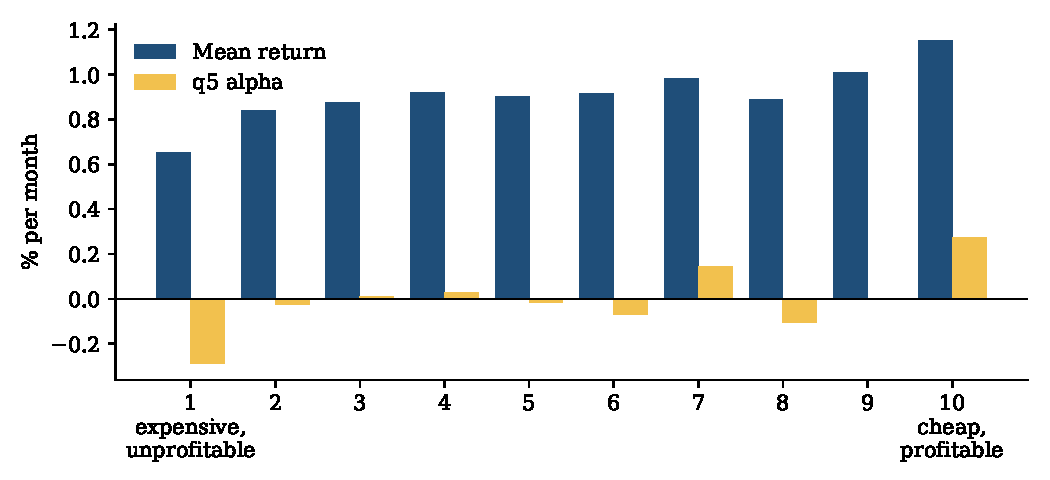
\includegraphics[width=0.85\textwidth]{figures/fig_deciles}
\caption{Average return and q5 alpha of the ten value-weighted portfolios, 1963--2015 (\% per
month).}\label{fig:deciles}
\end{figure}

\subsection{The long-short strategy}

Table~\ref{tab:spread} reports the long-short spread. Value-weighted, it earns 0.50\% per month
before and 0.33\% after trading costs ($t=2.61$). Turnover is about 9\% of each side per month and
trading costs 0.17\% per month on average: 0.23\% in 1963--1994 and 0.09\% in 1995--2015, as spreads
have narrowed. Against every model the net alpha is positive and significant over 1963--2015: 0.42\%
for the CAPM, 0.36\% for FF5, 0.53\% for FF6, 0.41\% for q5 and 0.36\% for q5+STR. The FF6 alpha is
higher than the raw return because the strategy loads negatively on the market and on momentum
(Section~\ref{sec:behaviour}); the q5 alpha, which does not depend on a momentum factor, confirms the
result.

The alpha is stronger in the second half of the sample. In 1963--1994 the strategy earns a
significant CAPM alpha (0.35\%, $t=2.45$), while the Fama-French factors explain most of its return;
in 1995--2015 it earns an FF6 alpha of 0.77\% ($t=4.03$) and a q5 alpha of 0.62\% ($t=2.81$).
Figure~\ref{fig:rolling} shows the same pattern over rolling ten-year windows: the six-factor alpha is
positive in 80\% of all windows and lies between about 6\% and 13.5\% per year in every window
ending from December 2000 onwards. The window ending in 2000 is instructive: the net return is $-4.1\%$ per year, as
expensive technology stocks kept rising, but the six-factor alpha is $+6.2\%$, so the loss came from
factor exposures, not from the stock selection.

\begin{table}[H]
\centering
\caption{Long-short spread (decile 10 minus decile 1), 1963--2015}\label{tab:spread}
\begin{tabular}{lrrr}
\toprule
 & 1963--2015 & 1963--1994 & 1995--2015 \\
\midrule
\multicolumn{4}{l}{\textit{Panel A: value-weighted}} \\
Gross return & 0.50 (3.96) & 0.50 (3.38) & 0.50 (2.22) \\
Net return & 0.33 (2.61) & 0.27 (1.85) & 0.41 (1.84) \\
CAPM net $\alpha$ & 0.42 (3.44) & 0.35 (2.45) & 0.52 (2.40) \\
FF5 net $\alpha$ & 0.36 (2.55) & -0.06 (-0.50) & 0.55 (2.26) \\
FF6 net $\alpha$ & 0.53 (3.77) & 0.02 (0.12) & 0.77 (4.03) \\
q5 net $\alpha$ & 0.41 (2.58) & 0.24 (1.33) & 0.62 (2.81) \\
q5+STR net $\alpha$ & 0.36 (2.27) & 0.21 (1.14) & 0.59 (2.67) \\
Turnover (\% per side) & 8.8 & 9.0 & 8.6 \\
Trading cost (\%) & 0.17 & 0.23 & 0.09 \\
\midrule
\multicolumn{4}{l}{\textit{Panel B: equal-weighted}} \\
Gross return & 0.64 (5.79) & 0.58 (4.94) & 0.74 (3.44) \\
Net return & 0.08 (0.69) & -0.06 (-0.45) & 0.28 (1.32) \\
CAPM net $\alpha$ & 0.16 (1.31) & 0.01 (0.06) & 0.40 (1.68) \\
FF5 net $\alpha$ & -0.22 (-2.05) & -0.43 (-3.65) & -0.05 (-0.26) \\
FF6 net $\alpha$ & 0.03 (0.29) & -0.20 (-1.79) & 0.17 (1.40) \\
q5 net $\alpha$ & -0.01 (-0.09) & 0.15 (1.03) & 0.04 (0.20) \\
q5+STR net $\alpha$ & -0.06 (-0.43) & 0.03 (0.22) & 0.04 (0.17) \\
Turnover (\% per side) & 12.5 & 12.3 & 12.8 \\
Trading cost (\%) & 0.56 & 0.63 & 0.46 \\
\bottomrule
\end{tabular}

\tablenote{Monthly returns and alphas in \%, $t$-statistics in parentheses (Newey-West, six lags).
Alphas are estimated on the net spread. Turnover is the average one-way monthly turnover of the long
and short portfolios; trading cost is the monthly cost of both sides.}
\end{table}

\begin{figure}[H]
\centering
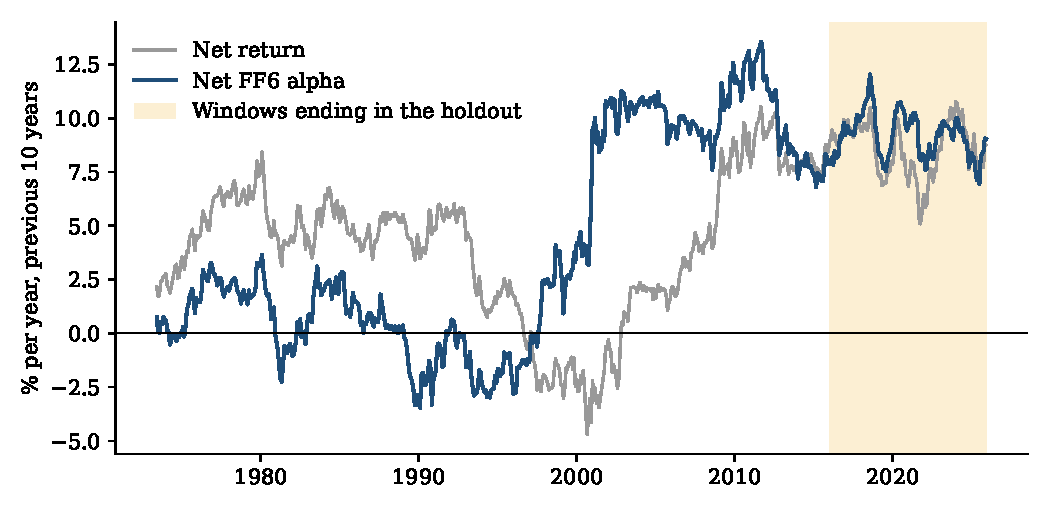
\includegraphics[width=0.9\textwidth]{figures/fig_rolling}
\caption{Net return and net six-factor alpha of the value-weighted long-short spread over the
previous ten years, annualised (\% per year). The shaded area marks windows that end in the holdout
period.}\label{fig:rolling}
\end{figure}

\subsection{Value- versus equal-weighting}

Equal-weighted, the gross spread is larger (0.64\%, $t=5.79$) but the net spread is only 0.08\% and
no net alpha is significant (Panel B of Table~\ref{tab:spread}). Equal weights give much more weight
to small stocks, which have wider spreads and less volume, and require trading every month to restore
the weights: costs are 0.56\% per month. The strategy is therefore a large-cap strategy, which is
also where a fund can implement it.

\subsection{Building the strategy step by step}

Table~\ref{tab:blocks} adds the three corrections one at a time, in the same universe and with the
same cost model. The first row sorts stocks on value and quality across the whole market. It earns
the highest net return, 0.57\% per month, but most of it is exposure to known factors: the FF6 alpha
is 0.24\% ($t=1.75$) and the q5 alpha 0.06\%. Ranking within industries lowers the raw return to
0.38\% but raises the FF6 alpha to 0.35\%: the industry bet of the plain sort earned returns that the
factors explain. Adding intangible capital to book value raises the return to 0.45\%, and adding it
to profitability raises the alphas (FF6 0.45\%, $t=3.13$; q5 0.24\%). Finally, measuring cheapness at
the current price and forming portfolios every three months raises the FF6 alpha to 0.53\% and the
q5 alpha to 0.41\% ($t=2.58$).

Overall, the corrections trade raw return for alpha: from the first to the last row the net return
falls from 0.57\% to 0.33\%, while the six-factor and q5 alphas rise at every step, from 0.24\% to
0.53\% and from 0.06\% to 0.41\%. The five-factor alpha does not: it falls from 0.50\% to 0.36\% in
the last step. They remove from the signal the parts of value and quality that the factors
already price. An investor who only holds the market and wants the highest stand-alone return could
prefer the annual version; a manager whose benchmark already contains the Fama-French and q-factors,
and who is paid for alpha, prefers the final one. We take the second view.

\begin{table}[H]
\centering
\caption{Building the strategy one correction at a time, 1963--2015}\label{tab:blocks}
\resizebox{\textwidth}{!}{\begin{tabular}{lrrrr}
\toprule
 & Net return & FF5 net $\alpha$ & FF6 net $\alpha$ & q5 net $\alpha$ \\
\midrule
Value + quality, ranked across all stocks & 0.57 (3.66) & 0.32 (2.40) & 0.24 (1.75) & 0.06 (0.35) \\
+ ranked within industries & 0.38 (2.95) & 0.37 (2.83) & 0.35 (2.31) & 0.15 (0.97) \\
+ intangible capital in book value & 0.45 (3.57) & 0.42 (3.32) & 0.36 (2.64) & 0.16 (1.15) \\
+ intangible capital in profitability & 0.46 (3.64) & 0.50 (3.78) & 0.45 (3.13) & 0.24 (1.60) \\
+ current prices, formed every 3 months (final) & 0.33 (2.61) & 0.36 (2.55) & 0.53 (3.77) & 0.41 (2.58) \\
\bottomrule
\end{tabular}
}
\tablenote{Value-weighted decile spread (10--1) after trading costs, \% per month, $t$-statistics in
parentheses (Newey-West, six lags for the alphas). Same universe (no microcaps), cost model and
sample in every row. The first four rows use the December price and form portfolios once a year, at
the end of June; the last row is the final strategy.}
\end{table}

\subsection{Out-of-sample: the 2016--2025 holdout}\label{sec:holdout}

Table~\ref{tab:holdout} reports the single evaluation of the holdout. The strategy did better out of
sample than in sample: the value-weighted net return is 0.73\% per month ($t=2.17$) and the net
alphas are 0.95\% for the CAPM, 0.75\% for FF6 and 0.58\% for q5 ($t=2.41$), all significant despite
only 120 months. Trading costs were only 0.02\% per month, as spreads are narrow today. The strategy
gained in eight of the ten years, including 2018 (+16\%) and 2022 (+10\%), when the market fell
(Figure~\ref{fig:years}). Over the whole period 1963--2025 the net return is 0.39\% per month
($t=3.31$), with an FF6 alpha of 0.58\% ($t=4.78$) and a q5 alpha of 0.36\% ($t=2.45$). Ten years
remain a short sample: we read the holdout as evidence that the effect did not disappear after our
research period, rather than as a precise estimate of its future size.

\begin{table}[H]
\centering
\caption{The holdout period 2016--2025}\label{tab:holdout}
\begin{tabular}{lrrr}
\toprule
 & 1963--2015 & 2016--2025 (holdout) & 1963--2025 \\
\midrule
\multicolumn{4}{l}{\textit{Panel A: value-weighted}} \\
Gross return & 0.50 (3.96) & 0.75 (2.23) & 0.54 (4.54) \\
Net return & 0.33 (2.61) & 0.73 (2.17) & 0.39 (3.31) \\
CAPM net $\alpha$ & 0.42 (3.44) & 0.95 (3.58) & 0.50 (4.41) \\
FF5 net $\alpha$ & 0.36 (2.55) & 0.70 (2.32) & 0.42 (3.54) \\
FF6 net $\alpha$ & 0.53 (3.77) & 0.75 (2.66) & 0.58 (4.78) \\
q5 net $\alpha$ & 0.41 (2.58) & 0.58 (2.41) & 0.36 (2.45) \\
q5+STR net $\alpha$ & 0.36 (2.27) & 0.61 (2.57) & 0.32 (2.15) \\
Net Sharpe ratio (annual) & 0.36 & 0.69 & 0.42 \\
\midrule
\multicolumn{4}{l}{\textit{Panel B: equal-weighted}} \\
Gross return & 0.64 (5.79) & 0.41 (1.25) & 0.60 (5.66) \\
Net return & 0.08 (0.69) & 0.26 (0.80) & 0.11 (0.99) \\
CAPM net $\alpha$ & 0.16 (1.31) & 0.41 (1.21) & 0.20 (1.74) \\
FF5 net $\alpha$ & -0.22 (-2.05) & 0.14 (0.63) & -0.16 (-1.69) \\
FF6 net $\alpha$ & 0.03 (0.29) & 0.19 (0.88) & 0.06 (0.73) \\
q5 net $\alpha$ & -0.01 (-0.09) & 0.16 (0.64) & -0.03 (-0.23) \\
q5+STR net $\alpha$ & -0.06 (-0.43) & 0.19 (0.75) & -0.08 (-0.68) \\
Net Sharpe ratio (annual) & 0.10 & 0.25 & 0.13 \\
\bottomrule
\end{tabular}

\tablenote{Monthly returns and net alphas in \%, $t$-statistics in parentheses (Newey-West, six lags).
The 2016--2025 period was evaluated once, with the rules fixed on 1963--2015
(Section~\ref{sec:method}). Sharpe ratio of the net spread, annualised.}
\end{table}

\subsection{Portfolio implications}\label{sec:portfolio}

From the perspective of a fund manager, the relevant question is whether the strategy improves a
portfolio. Run alone as a market-neutral fund, with the capital in T-bills and the long-short spread
on top, it earns 8.4\% per year with a volatility of 10.9\% and a maximum drawdown of $-24\%$ over
1963--2015, against 10.1\%, 15.3\% and $-50\%$ for the stock market. As a market-neutral fund it grows
less than the market, which carries full equity risk. Because its correlation with the market is
$-0.26$, however, adding it to a market portfolio as an overlay (the market plus one unit of the net
long-short spread) raises the Sharpe ratio from 0.39 to 0.61 over the same period and raises the
final wealth (Figure~\ref{fig:growth}).

\begin{figure}[H]
\centering
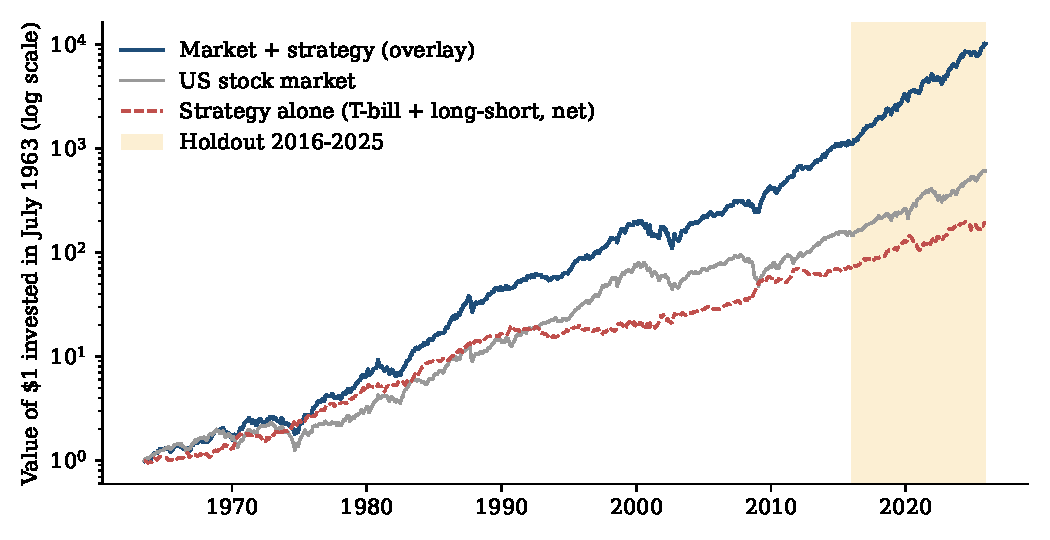
\includegraphics[width=0.9\textwidth]{figures/fig_growth}
\caption{Value of \$1 invested in July 1963, log scale: the US stock market, the market with the
long-short strategy added as an overlay (market plus one unit of the net long-short spread), and the
strategy alone as a market-neutral fund (T-bill plus the net spread). The shaded area is the holdout
period.}\label{fig:growth}
\end{figure}

% =====================================================================================
\section{Robustness}\label{sec:robust}

\subsection{Universe and formation frequency}

Table~\ref{tab:robust} varies the main choices. Including microcaps raises the q5 alpha to 0.45\%
($t=2.99$); restricting the universe to stocks above the NYSE median gives 0.30\% ($t=1.99$), with
an FF6 alpha of 0.48\% ($t=3.47$). Forming portfolios every month or every six months gives q5 alphas
of 0.36\% and 0.39\%, close to the 0.41\% of the three-month choice, so the result does not depend on
the precise holding period. A turnover buffer that keeps a stock in the long (short) portfolio while
it stays in the top (bottom) three deciles cuts turnover from 8.8\% to 3.5\% per month.

\begin{table}[H]
\centering
\caption{Robustness: universe and formation frequency, 1963--2015}\label{tab:robust}
\resizebox{\textwidth}{!}{\begin{tabular}{lrrrr}
\toprule
 & Net return & FF6 net $\alpha$ & q5 net $\alpha$ & Turnover \\
\midrule
Main specification & 0.33 (2.61) & 0.53 (3.77) & 0.41 (2.58) & 8.8 \\
With microcaps & 0.37 (3.01) & 0.55 (4.14) & 0.45 (2.99) & 8.9 \\
Large caps only (above NYSE median) & 0.29 (2.29) & 0.48 (3.47) & 0.30 (1.99) & 8.6 \\
Formed every month & 0.25 (2.02) & 0.46 (3.50) & 0.36 (2.34) & 14.1 \\
Formed every 6 months & 0.29 (2.35) & 0.48 (3.30) & 0.39 (2.36) & 6.6 \\
Every 3 months + turnover buffer & 0.32 (2.80) & 0.38 (3.41) & 0.25 (1.98) & 3.5 \\
\bottomrule
\end{tabular}
}
\tablenote{Value-weighted long-short spread after trading costs, \% per month, $t$-statistics in
parentheses. Turnover in \% per side and month.}
\end{table}

\subsection{Trading costs and capacity}

Table~\ref{tab:costs} varies the cost model and the size of the fund. With the spread only, the q5
alpha is 0.42\%; the price impact of a \$100 million fund lowers it by only 0.01\%, and a square-root
impact function gives the same result. The alpha declines with fund size but remains significant up
to \$500 million per side (q5 alpha 0.35\%, $t=2.22$). Allowing five days to execute each rebalancing
brings costs down to the level of the spread alone.

\begin{table}[H]
\centering
\caption{Trading costs and fund size, 1963--2015}\label{tab:costs}
\begin{tabular}{lrrrr}
\toprule
Cost model / fund size per side & Cost & Net return & FF6 net $\alpha$ & q5 net $\alpha$ \\
\midrule
Half spread only & 0.15 & 0.35 (2.76) & 0.55 (3.91) & 0.42 (2.67) \\
Linear impact, \$10m & 0.16 & 0.34 (2.75) & 0.55 (3.89) & 0.42 (2.66) \\
Linear impact, \$100m (main) & 0.17 & 0.33 (2.61) & 0.53 (3.77) & 0.41 (2.58) \\
Square-root impact, \$100m & 0.18 & 0.33 (2.59) & 0.53 (3.76) & 0.40 (2.56) \\
Linear impact, \$500m & 0.24 & 0.26 (2.05) & 0.46 (3.27) & 0.35 (2.22) \\
Linear impact, \$1bn & 0.33 & 0.17 (1.36) & 0.37 (2.65) & 0.28 (1.79) \\
Linear impact, \$2.5bn & 0.56 & -0.06 (-0.45) & 0.14 (0.97) & 0.09 (0.55) \\
Linear impact, \$100m, 5 days to trade & 0.16 & 0.34 (2.73) & 0.55 (3.88) & 0.42 (2.65) \\
\bottomrule
\end{tabular}

\tablenote{Value-weighted long-short spread, \% per month, $t$-statistics in parentheses. Fund size
per side in December 2025 dollars, scaled back in time with the market's dollar volume. Cost is the
monthly trading cost of both sides.}
\end{table}

\subsection{Luck and overfitting}\label{sec:overfit}

Beyond the holdout, we run three checks. First, a block bootstrap with 12-month blocks gives a 95\%
confidence interval for the mean net return of 0.09\% to 0.59\% per month, and leaving out any
single year keeps the $t$-statistic between 2.28 and 2.89.

Second, a placebo test (Table~\ref{tab:overfit}, Panel A): we shuffle the score randomly across
stocks within each month, 20 times, and run exactly the same code. If the alpha came from the
backtesting procedure itself, for instance through a look-ahead bias or a hidden size or industry
tilt, the placebos would show it too. They do not: their average gross q5 alpha is 0.01\% and the
highest is below 0.20\%, against 0.56\% for the real score.

Third, we split the stocks randomly into two halves, three times, and run the strategy on each half
separately (Panel B). The net FF6 alpha is significant in all six halves and the net q5 alpha is
positive in all six, so the result is not driven by a small group of stocks. Together with the
stability across neighbouring specifications in Table~\ref{tab:robust} and the holdout, these checks
indicate that the strategy captures a genuine effect rather than a feature of our sample.

\begin{table}[H]
\centering
\caption{Placebo and random-half tests, 1963--2015}\label{tab:overfit}
\resizebox{\textwidth}{!}{\begin{tabular}{lrrrr}
\toprule
 & Real & Placebo mean & Placebo 5\% & Placebo 95\% \\
\midrule
\multicolumn{5}{l}{\textit{Panel A: placebo, score shuffled across stocks within each month (gross, VW)}} \\
Gross return & 0.50 & 0.02 & -0.09 & 0.10 \\
FF6 $\alpha$ & 0.71 & 0.01 & -0.11 & 0.08 \\
q5 $\alpha$ & 0.56 & 0.01 & -0.23 & 0.18 \\
\midrule
\multicolumn{5}{l}{\textit{Panel B: random halves of the stocks (net of costs, VW)}} \\
Split / half & Net return & FF6 net $\alpha$ & q5 net $\alpha$ &  \\
1 / A & 0.35 & 0.53 (3.08) & 0.43 (2.14) &  \\
1 / B & 0.25 & 0.43 (3.18) & 0.25 (1.68) &  \\
2 / A & 0.41 & 0.61 (3.71) & 0.47 (2.63) &  \\
2 / B & 0.22 & 0.43 (2.88) & 0.35 (1.98) &  \\
3 / A & 0.34 & 0.40 (2.64) & 0.22 (1.18) &  \\
3 / B & 0.28 & 0.54 (3.30) & 0.47 (2.66) &  \\
\bottomrule
\end{tabular}
}
\tablenote{Panel A: gross value-weighted spread and alphas (\% per month) of the real score and of 20
placebo scores obtained by shuffling the score across stocks within each month. Panel B: the strategy
run separately on two random halves of the stocks (three random splits), after trading costs;
$t$-statistics in parentheses.}
\end{table}

\subsection{Risk exposures and behaviour in crises}\label{sec:behaviour}

Table~\ref{tab:loadings} shows the six-factor loadings. The strategy has a negative market beta
($-0.15$), a positive loading on the investment factor CMA (0.40), as expected for firms that are
cheap and generate cash, and a negative loading on momentum ($-0.23$): cheap stocks are often recent
losers, the usual negative correlation between value and momentum
\citep{AsnessMoskowitzPedersen2013}. Its loading on HML is negative ($-0.20$): within-industry,
intangible-adjusted cheapness at current prices is a different measure from the standard
book-to-market, and the cheap firms it selects are not the ones HML buys.

Table~\ref{tab:conditional} shows when the strategy earns its returns. It loses 0.29\% per month when
the market rises and earns 1.19\% when it falls, 2.09\% in the 10\% worst market months and 1.17\% in
NBER recessions. Its best years are crises: 1970, 2001, 2008 and 2011.

\begin{table}[H]
\centering
\caption{Six-factor loadings of the net spread, 1963--2015}\label{tab:loadings}
\begin{tabular}{lrr}
\toprule
FF6 regression & Coefficient & $t$ \\
\midrule
$\alpha$ (\% per month) & 0.53 & (3.77) \\
Market & -0.15 & (-3.54) \\
SMB (size) & -0.10 & (-1.69) \\
HML (value) & -0.20 & (-2.35) \\
RMW (profitability) & 0.03 & (0.36) \\
CMA (investment) & 0.40 & (3.34) \\
MOM (momentum) & -0.23 & (-3.67) \\
$R^2$ & 0.19 &  \\
\bottomrule
\end{tabular}

\tablenote{Regression of the net value-weighted spread on the six factors, Newey-West $t$-statistics
(six lags).}
\end{table}

\begin{table}[H]
\centering
\caption{Returns in good and bad markets, 1963--2015}\label{tab:conditional}
\begin{tabular}{lrrr}
\toprule
Months & Strategy (\%) & Market excess (\%) & N \\
\midrule
Market up & -0.29 & 3.38 & 368 \\
Market down & 1.19 & -3.54 & 262 \\
10\% worst market months & 2.09 & -8.03 & 63 \\
NBER recessions & 1.17 & -0.82 & 90 \\
Expansions & 0.19 & 0.72 & 540 \\
All months & 0.33 & 0.50 & 630 \\
\bottomrule
\end{tabular}

\tablenote{Average net value-weighted spread and average market excess return (\% per month) in
months grouped by the market's return and by NBER business cycles.}
\end{table}

% =====================================================================================
\section{Limitations}\label{sec:limits}

Four aspects should be kept in mind. First, the alpha against the multifactor models is concentrated
after 1995 and in the holdout; before 1995 the Fama-French factors explain most of the return.
Second, a large part of the return is earned in crises, so the strategy works best as a hedge and
can lag the market in strong bull markets. Third, it is a value-weighted, large-cap strategy:
equal-weighted, trading costs absorb the return. Fourth, our cost model does not include the fee for
borrowing the stocks sold short. The short leg holds large, liquid stocks: \citet{DAvolio2002} finds
that 91\% of the stocks on loan are general collateral, with an average fee of 0.17\% per year, which
would cost the short side about 0.015\% per month, small compared with the alpha.

% =====================================================================================
\section{Conclusion}\label{sec:conclusion}

We show that value and quality, measured within industries, corrected for intangible capital and at
current prices, earn a net alpha against the Fama-French and q-factor models after realistic trading
costs. Taken together, the corrections lower the part of the return that the factors explain, and
each one raises the six-factor and q5 alphas.
Over 1963--2015 the value-weighted strategy earns 0.33\% per month net of costs, with a six-factor
alpha of 0.53\% and a q5 alpha of 0.41\%, and on a holdout period evaluated once it earns 0.73\% with
a q5 alpha of 0.58\%. The result survives changes in the universe, the formation frequency and the
cost model, a placebo test and random splits of the stocks, and the strategy can be run by a fund of
up to about \$500 million per side. For a fund manager its main value is as a complement to the
market: it pays off when the market falls and, added as an overlay, raises the Sharpe ratio of a
market portfolio. Natural extensions are a direct measure of borrowing costs, a test in international
markets, and a combination with momentum, whose negative correlation with our signal could smooth
its returns.

\newpage
\printbibliography

\newpage
\appendix
\section{Additional figures}\label{app:figures}

\begin{figure}[H]
\centering
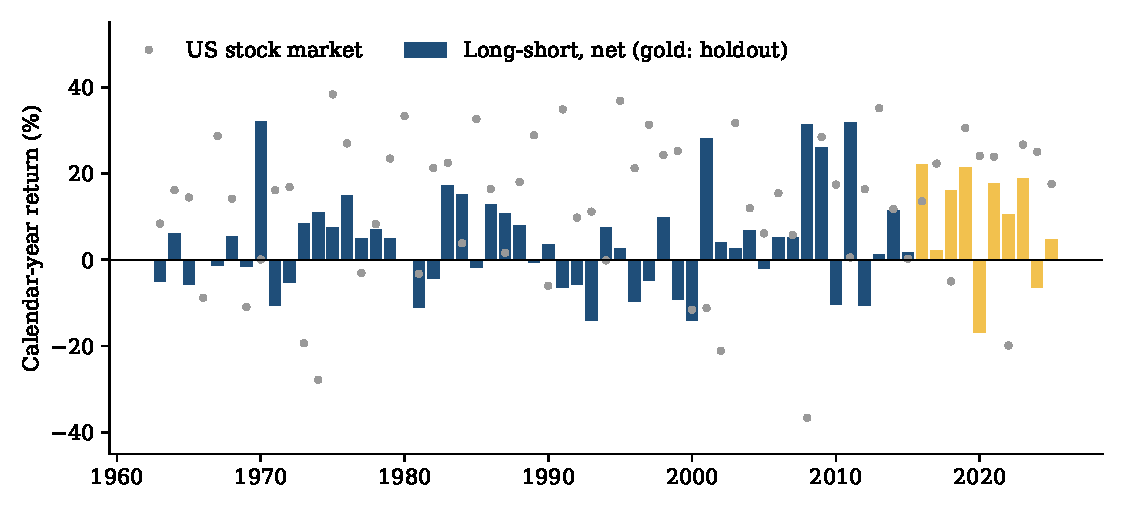
\includegraphics[width=0.95\textwidth]{figures/fig_years}
\caption{Calendar-year return of the long-short strategy after trading costs (bars; holdout years in
gold) and of the US stock market (dots), 1963--2025.}\label{fig:years}
\end{figure}

\end{document}
